\documentclass{article}
\usepackage{algpseudocode}
\usepackage[ruled]{algorithm}
\usepackage{url}
\usepackage{framed}
\usepackage{amsfonts,amsmath,amsthm,amssymb}
\usepackage{graphicx}
\usepackage{url}
\usepackage{color}
\usepackage{geometry}

\geometry{margin=1.2in}

\newcommand {\mean} {\ensuremath {\mathop{\mathrm{mean}}}}
\newcommand {\median} {\ensuremath {\mathop{\mathrm{median}}}}
\newcommand {\N} {\ensuremath {\mathcal{N}}}
\newcommand {\IE} {\ensuremath {\mathbb{E}}}
\newcommand {\cov} {\ensuremath {\mathop{\mathrm{cov}}}}
\newcommand {\BEL} {\ensuremath {\mathop{\mathrm{BEL}}}}

\newtheorem{lemma}{Lemma}

\title{Doing Better Than UCT: \\ Rational Monte Carlo Sampling in Trees}
\author {David Tolpin, Solomon Eyal Shimony \\
Department of Computer Science, \\
Ben-Gurion University of the Negev, Beer Sheva, Israel \\
\{tolpin,shimony\}@cs.bgu.ac.il}

\begin{document}

\maketitle

\begin{abstract}
UCT, a state-of-the art algorithm for Monte Carlo tree sampling
(MCTS), is based on UCB, a sampling policy for the Multi-armed Bandit
Problem (MAB) that minimizes the accumulated regret. However, MCTS
differs from MAB in that only the final choice, rather than all arm
pulls, brings a reward, that is, the simple regret, as opposite to the
accumulated regret, must be minimized. This work introduces policies for
multi-armed bandits with lower simple regret than UCB, and an
algorithm for MCTS which combines accumulated and simple regret
minization and outperforms UCT. Finite-time and asymptotic analysis of
the policies is provided, and the algorithms are empirically compared.
\end{abstract}


\section{Introduction}

The simple regret of a sampling policy for the Multi-armed Bandit
Problem is the expected difference between the best expected reward
$\mu_*$ and the expected reward of the arm with the best sample mean
$\mu_j,\;\overline X_j=\max_i\overline X_i$:
\begin{equation}
\label{eq:simple-regret}
\IE[R]=\sum_{j=1}^K\Delta_j\Pr(\overline X_j=\max_i\overline X_i)
\end{equation}
where $\Delta_j=\mu_*-\mu_j$.

\section{Main Results}

\subsection{Doing better than UCB}

\begin{figure}[t]
  \centering
  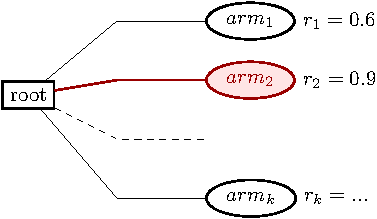
\includegraphics[scale=1.2]{onelevel-tree.pdf}
  \caption{Simple regret in MAB: the best arm}
  \label{fig:onelevel-tree}
\end{figure}

\begin{figure}[t]
  \centering
  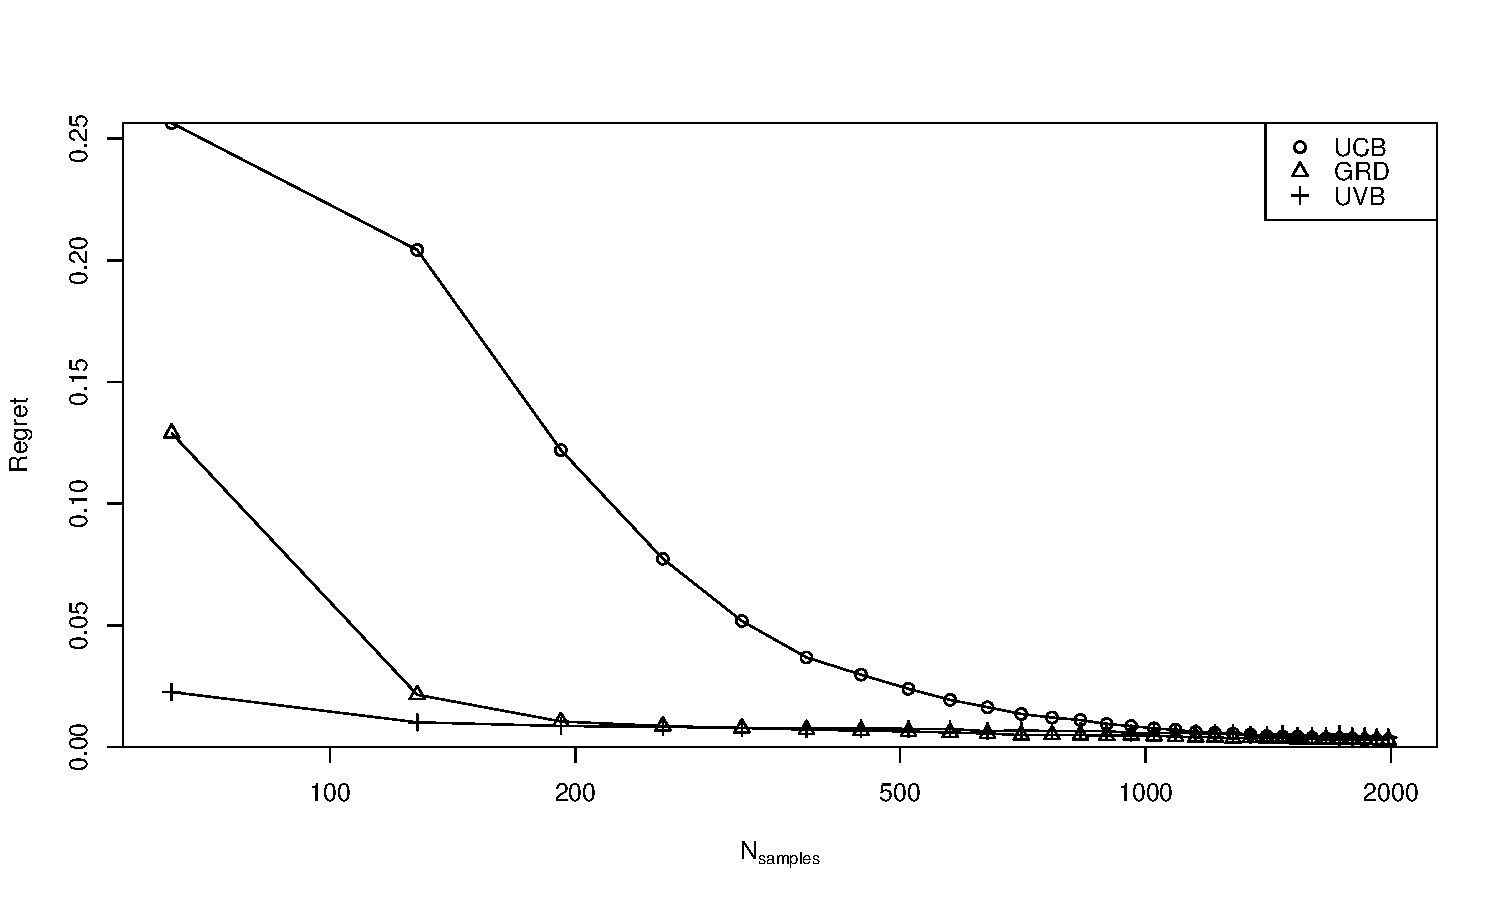
\includegraphics[scale=0.64]{onelevel-64.pdf}
  \caption{Simple regret in MAB: UCB vs. $\varepsilon$-greedy vs. Random}
  \label{fig:onelevel-64}
\end{figure}


\subsection{Doing better than UCT}

\begin{figure}[t]
  \centering
  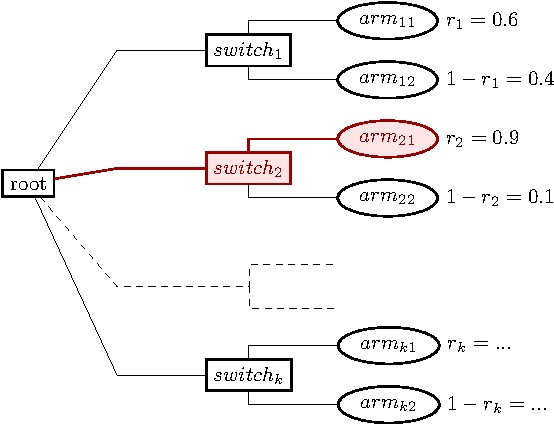
\includegraphics[scale=1.2]{twolevel-tree.pdf}
  \caption{MCTS: a path to the best arm}
  \label{fig:twolevel-tree}
\end{figure}

\begin{figure}[t]
  \centering
  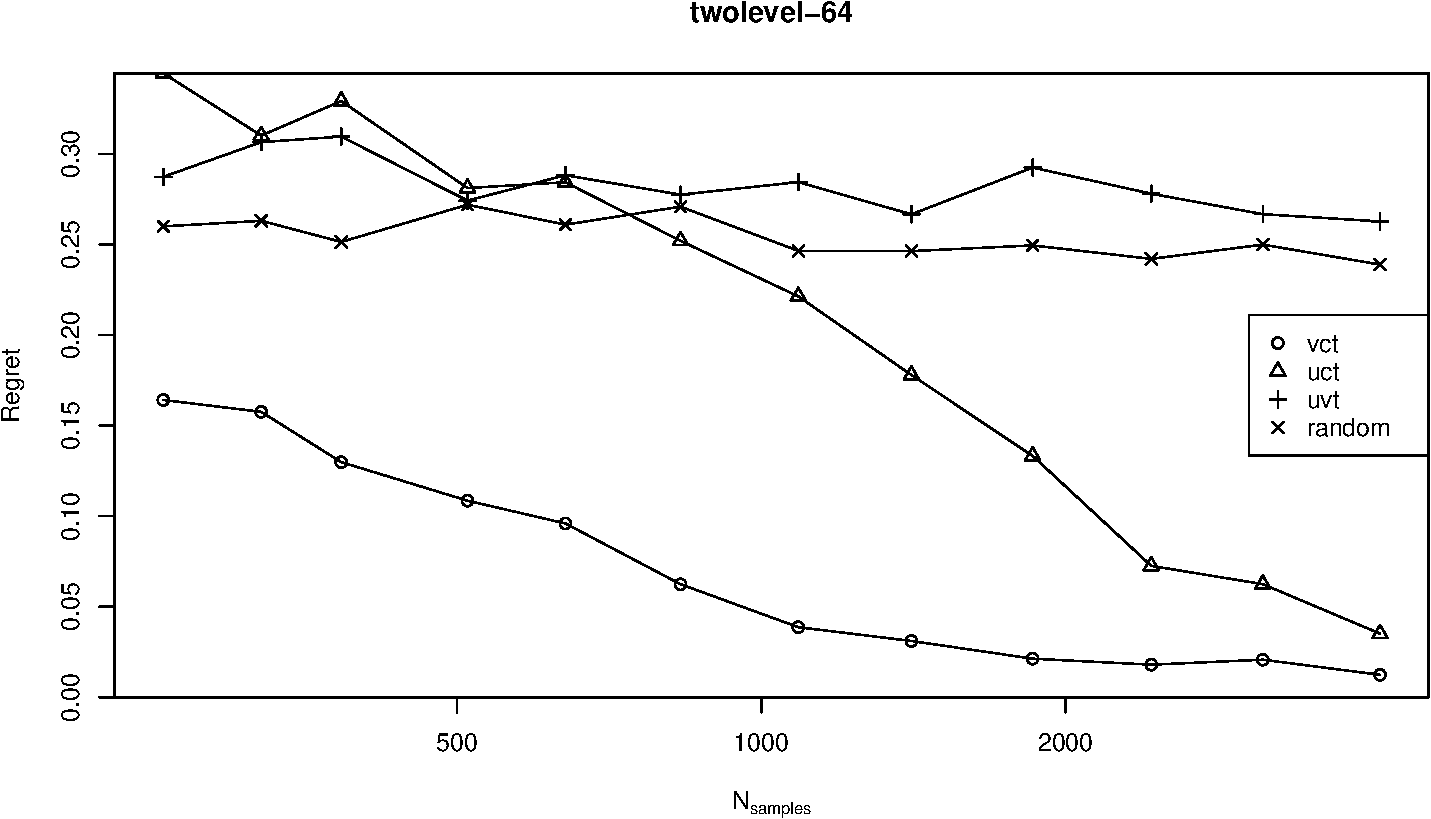
\includegraphics[scale=0.64,trim=0pt 0pt 0pt 24pt,clip]{twolevel-64.pdf}
  \caption{MCTS: UCT vs. GRT vs. GCT vs. Random}
  \label{fig:twolevel-64}
\end{figure}

\section{Empirical Evaluation}

\subsection{Monte Carlo tree search}

\begin{figure}[t]
  \centering
  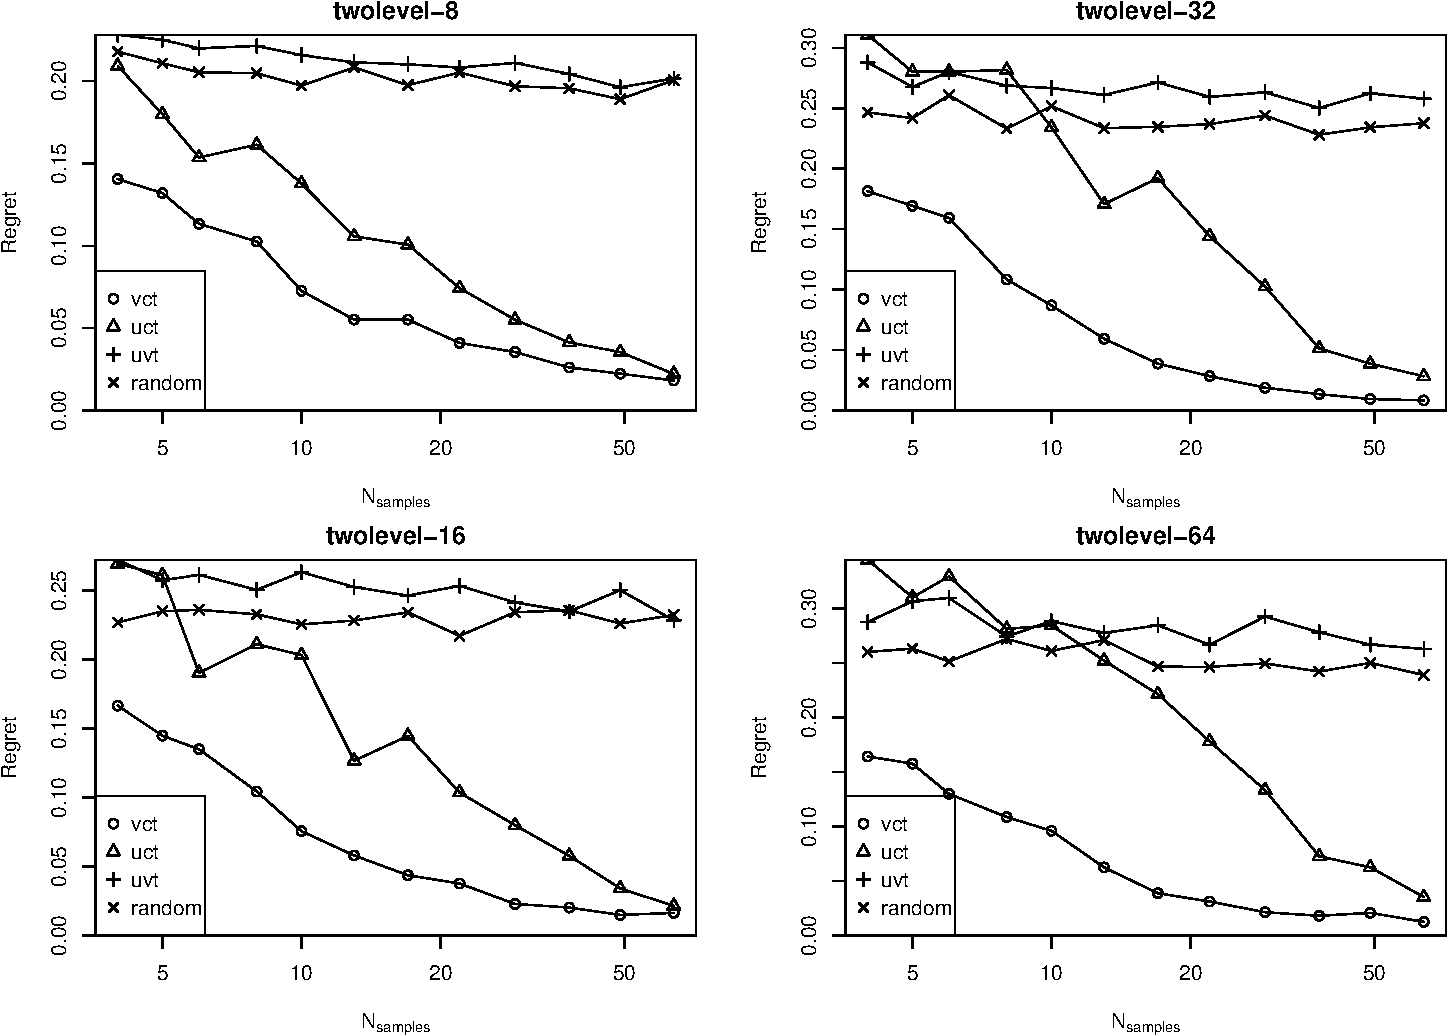
\includegraphics[scale=0.64,trim=0pt 0pt 0pt 0pt,clip]{twolevel-8-16-32-64.pdf}
  \caption{Monte carlo tree search, varying number of arms}
  \label{fig:twolevel-8-16-32-64}
\end{figure}

\subsection{The sailing domain}


\begin{figure}[t]
  \begin{minipage}[b]{0.5\linewidth} \centering
    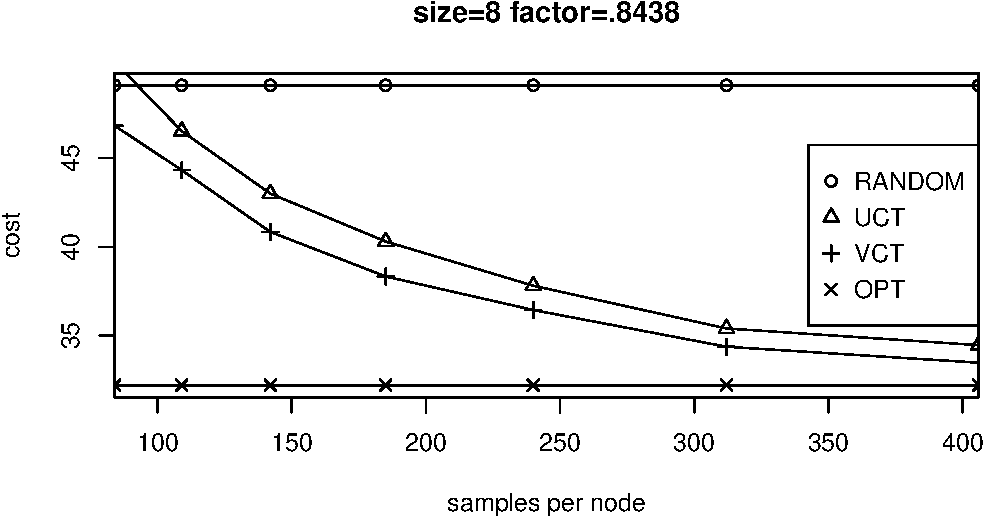
\includegraphics[scale=0.45,trim=0pt 0pt 0pt
    0pt,clip]{sailing-size=8-factor=_8438.pdf}
    {a. varying number of samples} 
 \end{minipage}
  \begin{minipage}[b]{0.5\linewidth} \centering
    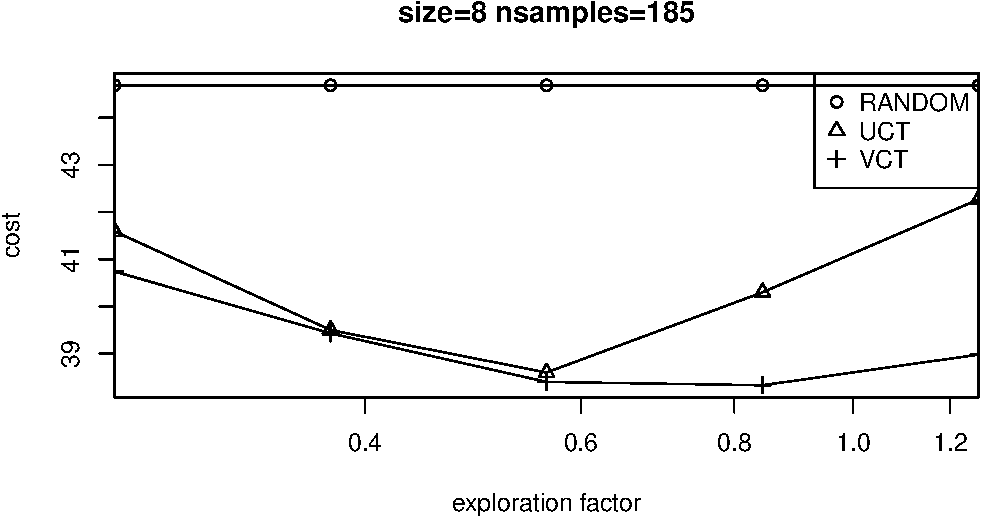
\includegraphics[scale=0.45,trim=0pt 0pt 0pt
    0pt,clip]{sailing-size=8-nsamples=185.pdf}
    {b. varying exploration factor}
  \end{minipage}
  \caption{The sailing domain, a smaller lake}
  \label{fig:sailing-8}
\end{figure}

\begin{figure}[t]
  \begin{minipage}[b]{0.5\linewidth} \centering
    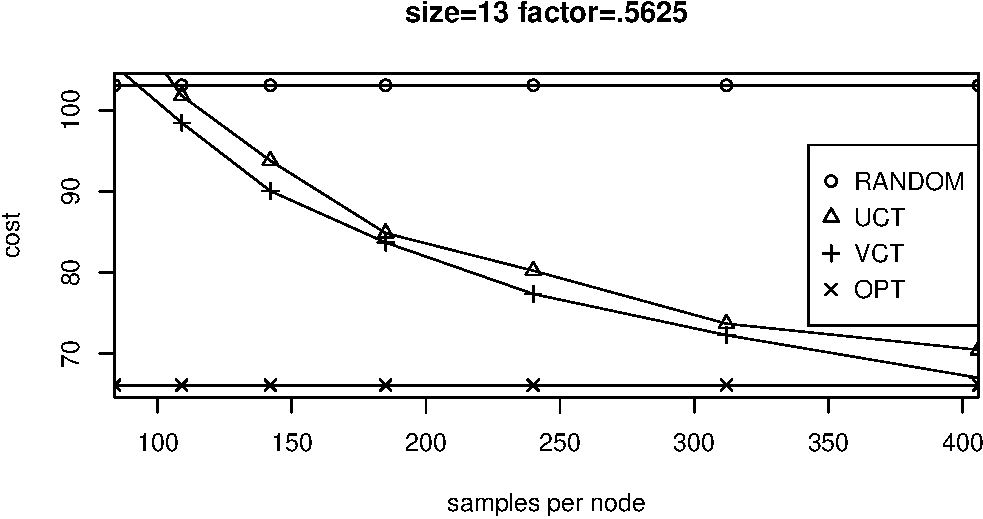
\includegraphics[scale=0.45,trim=0pt 0pt 0pt
    0pt,clip]{sailing-size=13-factor=_5625.pdf}
    {a. varying number of samples}
  \end{minipage}
  \begin{minipage}[b]{0.5\linewidth} \centering
    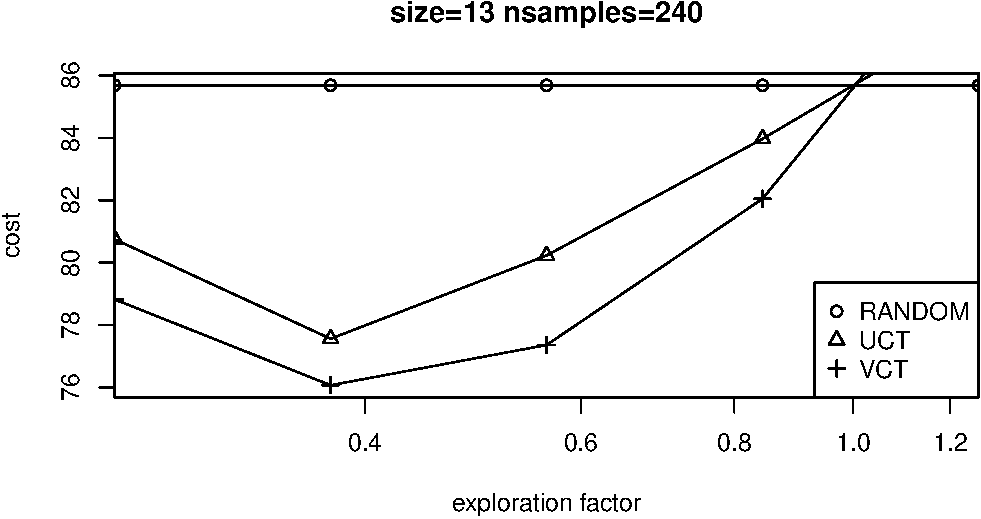
\includegraphics[scale=0.45,trim=0pt 0pt 0pt
    0pt,clip]{sailing-size=13-nsamples=240.pdf}
    {b. varying exploration factor}
  \end{minipage}
  \caption{The sailing domain, a larger lake}
  \label{fig:sailing-13}
\end{figure}

\section{Summary and Future Work}

\section*{Acknowledgments}

The research is partially supported by Israel
Science Foundation grant 305/09, by the Lynne and William Frankel
Center for Computer Sciences, and by the Paul Ivanier Center for
Robotics Research and Production Management.

\bibliographystyle{plain}
\bibliography{refs}

\pagebreak

\appendix

\section{Facts}

{\bf Chernoff bound (see \cite{Hagerup.chernoff}):} for $m$ independent random variables $X_1, X_2, ..., X_m$
taking values 0 or 1, $X=\sum_{i=1}^m X_i$, and $0\le\delta\le 1$:

\begin{equation}
\label{eq:chernoff-bound}
\Pr[X < (1-\delta)\IE[X]] < e^{-\delta^2\IE[X]/2}
\end{equation}

\section{Derivations}

\subsection{Finite-time regret bounds}

For an analysis of pure exploration of uniform and UCB algorithms, see also
\cite{Bubeck.pure}.


\subsubsection{$\varepsilon$-greedy}

For $0<\varepsilon\le1-\frac 1 K$ and $x_0>0$ (see Section 3, Proofs, in \cite{Auer.ucb}):

\begin{eqnarray}
\Pr(\overline X_j=\max_i\overline X_i)&\le&2\left(x_0\cdot \Pr\left\{T_j^R(n)\le x_0\right\} + \frac 2{\Delta_j^2}e^{-\Delta_j^2\lfloor x_0 \rfloor/2}\right)\nonumber\\
&\le&2\left(x_0\cdot \Pr\left\{T_j^R(n)\le x_0\right\} + \frac {2 \cdot
  e^{\Delta_j^2/2}}{\Delta_j^2}e^{-\Delta_j^2 x_0 /2}\right)
\end{eqnarray}

Number of times $\mu$ the $j$th arm is selected {\it randomly}:

\begin{equation}
\mu\triangleq\IE\left[T_j^R(n)\right]=\frac {n\varepsilon} K
\end{equation}

By choosing $x_0=\frac \mu 2$ and applying the Chernoff bound (\ref{eq:chernoff-bound}), obtain:

\begin{eqnarray}
\label{eq:pr-epsilon-greedy}
\Pr(\overline X_j=\max_i\overline X_i)&\le& 2\left(\frac {\mu}{2} e^{-\mu/8} + \frac {2e^{\Delta_j^2/2}}{\Delta_j^2}e^{-\Delta_j^2 \mu/4}\right)\nonumber\\
&\le&\left(\mu + \frac {4\sqrt e}{\Delta_j^2}\right)e^{-\Delta_j^2\mu/8}
\end{eqnarray}

A bound on the simple regret $R_\varepsilon$ of an
$\varepsilon$-greedy policy follows from substituting
(\ref{eq:pr-epsilon-greedy}) into (\ref{eq:simple-regret}):

\begin{eqnarray}
\IE[R_\varepsilon]&\le&\sum_{j=1}^K\Delta_j\left(\mu + \frac {4\sqrt e}
{\Delta_j^2}\right)e^{-\Delta_j^2\mu/8}\nonumber\\
&\le&K\left(\mu + \frac {4\sqrt e}{\Delta_{\min}}\right)e^{-\Delta_{\min}^2\mu/8}
\end{eqnarray}

\subsubsection{UCB}

Regret $R_{UCB}$:

\subsubsection{UVB}

Regret $R_{UVB}$:

\subsection{Asymptotic bounds for $\varepsilon$-greedy policies}

\end{document}
